\documentclass[11pt]{article}

\usepackage[utf8]{inputenc}
\usepackage[T1]{fontenc}
\usepackage[margin=1in]{geometry}
\usepackage{hyperref}
\usepackage{booktabs}
\usepackage{array}
\usepackage{tabularx}
\usepackage{listings}
\usepackage{xcolor}

\usepackage[numbers,sort&compress]{natbib}
\usepackage{amsmath}
\usepackage{tikz}
\usetikzlibrary{arrows.meta, positioning, shapes.geometric}

\hypersetup{
  colorlinks=true,
  linkcolor=blue!70!black,
  citecolor=blue!70!black,
  urlcolor=blue!70!black
}

\lstset{
  basicstyle=\ttfamily\small,
  breaklines=true,
  frame=single,
  backgroundcolor=\color{gray!8},
  rulecolor=\color{gray!40}
}

\title{\textbf{Synaptic Mesh: Receipt-Preserving Memory Authority\\for Multi-Agent Systems}\\[0.4em]
{\large A protocol proposal and local fixture evaluation}}

\author{
  Gabriel Pe\~{n}a\\
  \textit{Independent Researcher}\\
  \href{https://github.com/lechuit/synaptic-mesh}{\texttt{github.com/lechuit/synaptic-mesh}}
}

\date{May 2026}

\begin{document}

\maketitle

\begin{abstract}
Agent memory systems increasingly persist, retrieve, summarize, and share context across
tools, sessions, and specialized agents. Recent work on retrieval, agent memory,
policy provenance, and stateful frameworks has advanced retrieval, persistence,
reflection, personalization, access control, and state management
\cite{R01_Lewis2020_RAG, R02_Gao2023_RAGSurvey, R03_FerraioloKuhn1992_RBAC,
R04_Hu2014_ABAC, R07_MoreauMissier2013_PROVDM, R14_Packer2023_MemGPT,
R16_LangGraph2026_Persistence, R17_AWS2026_AgentCoreMemory, R18_GoogleCloud2026_MemoryBank}.
These mechanisms are useful but do not by themselves answer a narrower multi-agent
question: what authority survives when memory-derived summaries travel through
compression, handoff, and action-planning steps? A memory can be relevant, well-summarized,
and correctly sourced while still being stale, local-only, denied, partial-lineage,
human-required, or unsafe to use as action authority.

This paper introduces \textbf{Synaptic Mesh}, a protocol proposal for multi-agent memory
authority. Borrowing from provenance and authorization traditions
\cite{R03_FerraioloKuhn1992_RBAC, R04_Hu2014_ABAC, R07_MoreauMissier2013_PROVDM,
R08_OpenPolicyAgent2026_Docs}, the core claim is that memory claims should carry
compact authority/status/boundary receipts that survive transformations such as:
\emph{source result} $\to$ \emph{summary} $\to$ \emph{handoff} $\to$ \emph{next-action}
$\to$ \emph{action proposal}. Receipts bind source identity, freshness, scope,
promotion boundary, forbidden effects, later restrictive events, and the proposed
action boundary. The receiving agent checks these receipts before treating a
memory-derived summary as permission, readiness, or durable truth.

Within local hand-authored adversarial fixtures, receipt-through-transform catches
several memory laundering failures: sender-safe label overrides, boundary substring
smuggling, cross-source authority laundering, stale receipt reuse, and over-trust in
confidence or prose fields. The latest compressed-temporal fixture identifies an
11-field authority-critical receipt tuple that preserves zero unsafe allows and zero
false rejects within those local tests while reducing field count by 31.25\% relative
to a fuller audit receipt. These results are not production benchmarks; they are a
falsification ledger supporting a narrower protocol hypothesis: multi-agent memory
systems may need authority-preserving transforms, not only better retrieval.

The reference implementation and reproducibility package are available at
\url{https://github.com/lechuit/synaptic-mesh}.
\end{abstract}

\section{Introduction}

As multi-agent AI systems grow in complexity, memory becomes a shared resource
passed through chains of agents that observe, summarize, critique, plan, and act.
These agents often exchange compressed context rather than raw evidence. This creates
a subtle but consequential risk: by the time a memory-derived summary reaches an
acting agent, the authority conditions of the original evidence may have been silently
discarded.

The problem is not retrieval quality. Retrieval-Augmented Generation and related
techniques \cite{R01_Lewis2020_RAG, R02_Gao2023_RAGSurvey} are highly effective at
surfacing relevant context. The problem is what happens \emph{after} retrieval, during
the compression and handoff steps that prepare context for action planning. A summary
can be semantically accurate while omitting the fact that its source was local-only,
stale, partially denied, or conditioned on human approval. Recent empirical work
supports the broader concern: Liu et al.~\cite{R19_Liu2026_MemoryCurse} find that
expanding accessible memory history systematically degrades cooperative behavior in
LLM agents across 28 model-game settings, a result they term the ``memory curse.''
That work focuses on the \emph{quantity} of history; Synaptic Mesh addresses the
complementary structural problem of whether the \emph{authority} conditions embedded
in that history survive compression and handoff.

This paper introduces \textbf{Synaptic Mesh}, a protocol proposal for preserving
authority, scope, and boundary receipts through multi-agent memory transforms. The
central design maxim is:

\begin{quote}
\textit{Do not build a memory that remembers more.\\
Build a memory that knows when to distrust itself.}
\end{quote}

\subsection*{Contributions}

\begin{enumerate}
  \item We formalize \emph{memory laundering} as a distinct failure mode in
    multi-agent memory systems: authority-conditioned evidence being silently
    transformed into apparent permission through compression and handoff steps.
  \item We propose \emph{receipt-through-transform} as a protocol primitive: compact
    authority receipts that travel with compressed summaries and are checked by the
    receiver before acting.
  \item We identify a minimal 11-field authority-critical receipt tuple that, within
    local hand-authored fixtures, preserves zero unsafe allows and zero false rejects
    while reducing field count by 31.25\% relative to a fuller audit receipt.
  \item We evaluate the protocol against 12 classes of adversarial fixtures covering
    sender-label overrides, boundary smuggling, cross-source laundering, stale
    receipt reuse, and temporal precedence violations.
  \item We state explicit limitations, non-goals, and a threat model to bound the
    scope of the proposal and guide follow-on work.
\end{enumerate}

The paper proceeds as follows. Section~\ref{sec:problem} formalizes the memory
laundering failure model. Section~\ref{sec:architecture} presents the Synaptic Mesh
architecture. Section~\ref{sec:receipt} describes the receipt-through-transform
primitive. Section~\ref{sec:evidence} presents the local fixture evaluation.
Section~\ref{sec:related} situates the proposal relative to prior work.
Section~\ref{sec:threats} states the threat model and non-goals.
Section~\ref{sec:limitations} states limitations and future work.
Section~\ref{sec:conclusion} concludes.

\section{The Memory Laundering Problem}
\label{sec:problem}

\subsection{Failure model}

A multi-agent memory mesh fails when it:
\begin{enumerate}
  \item stores false or malicious content as stable fact;
  \item shares private memory with the wrong agent or scope;
  \item lets one weak or local claim become global authority;
  \item hides semantic conflicts under last-writer-wins summaries;
  \item compresses away evidence, boundary, or conditions;
  \item retrieves by superficial similarity instead of decision utility and authority;
  \item cannot preserve tombstones, rejection receipts, or later restrictive events;
  \item lets confidence, consensus, sender labels, or polished prose override
        source, freshness, scope, and boundary validation; or
  \item becomes too ceremonious and overblocks routine local work.
\end{enumerate}

Failure modes 4--8 constitute what we call \emph{memory laundering}: evidence whose
authority is conditioned on scope, freshness, approval, or explicit restrictions is
transformed into an apparent permission by the time it reaches an acting agent.

\subsection{Canonical laundering scenario}

\begin{enumerate}
  \item A source artifact marks a claim as local-only, stale, rejected, partial,
        or human-required.
  \item A summarizer compresses the useful part but drops the boundary qualifier.
  \item A handoff agent labels the result ``safe'' or ``ready.''
  \item A downstream receiver treats the summary as a permission signal.
  \item An action planner performs or proposes an effect the original evidence
        did not authorize.
\end{enumerate}

Classical retrieval relevance does not address this. A retrieved or summarized
result can be semantically relevant while still unauthorized for a proposed effect.
Access-control and zero-trust architectures \cite{R03_FerraioloKuhn1992_RBAC,
R04_Hu2014_ABAC, R05_Rose2020_ZeroTrust} separate possession of information from
permission to act on it, but their enforcement mechanisms assume a more static
subject-resource-action model than the dynamic multi-agent handoff context.
Provenance systems such as PROV-DM \cite{R07_MoreauMissier2013_PROVDM} track
derivation but do not by themselves prescribe how authority-critical fields should
be preserved through summarization. Policy engines \cite{R08_OpenPolicyAgent2026_Docs}
can evaluate allow/deny rules but still require that adequate memory lineage
reach the decision point.

\subsection{Worked example}
\label{sec:example}

Table~\ref{tab:example} shows a concrete laundering case and how Synaptic Mesh
addresses it within local hand-authored fixtures.

\begin{table}[h]
\centering
\caption{Worked laundering example: local-only policy claim promoted to publish action.}
\label{tab:example}
\begin{tabularx}{\textwidth}{@{}lX@{}}
\toprule
\textbf{Stage} & \textbf{Content} \\
\midrule
\textbf{Source artifact} &
``Policy draft v2: approved for internal review only. \textbf{Do not publish.}
Freshness: current. Scope: local\_shadow. Boundary: no\_promotion\_without\_human.'' \\
\addlinespace
\textbf{Defective summary} &
``Policy draft v2 is approved and current.'' \\
(boundary dropped) & \\
\addlinespace
\textbf{Dangerous handoff} &
``Policy draft v2 is ready. You may publish externally.'' \\
(sender overclaims) & \\
\addlinespace
\textbf{Correct receipt} &
\texttt{SRC=policy-draft-v2; FRESH=current; SCOPE=local\_shadow;} \\
& \texttt{PB=no\_promotion\_without\_human;} \\
& \texttt{NO=no\_external\_no\_publish; ACT=publish} \\
\addlinespace
\textbf{Receiver decision} &
Route: \texttt{ask\_human}. Reason codes: \texttt{EXTERNAL\_PUBLICATION\_PROMOTION},
\texttt{FREE\_TEXT\_NOT\_AUTHORITY}. Action \texttt{publish} blocked pending
explicit human approval. \\
\bottomrule
\end{tabularx}
\end{table}

Without the receipt, the receiver sees only the handoff prose and has no signal that
the proposed \texttt{publish} action exceeds the original source boundary. With the
receipt, the receiver independently classifies \texttt{ACT=publish} against
\texttt{NO=no\_publish} and routes to \texttt{ask\_human} regardless of how the
handoff was worded.

\section{Synaptic Mesh Architecture}
\label{sec:architecture}

\subsection{System flow}

\begin{figure}[h]
\centering
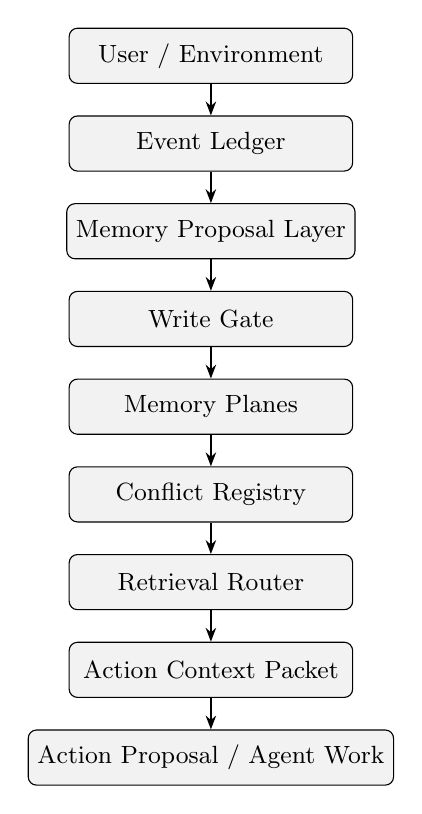
\begin{tikzpicture}[
  box/.style={draw, rounded corners=3pt, minimum width=3.6cm, minimum height=0.7cm,
              fill=gray!10, font=\small},
  arr/.style={-{Stealth[length=5pt]}, thick}
]
  \node[box] (env)    {User / Environment};
  \node[box] (ledger) [below=0.4cm of env]  {Event Ledger};
  \node[box] (prop)   [below=0.4cm of ledger] {Memory Proposal Layer};
  \node[box] (gate)   [below=0.4cm of prop]   {Write Gate};
  \node[box] (mem)    [below=0.4cm of gate]   {Memory Planes};
  \node[box] (conf)   [below=0.4cm of mem]    {Conflict Registry};
  \node[box] (router) [below=0.4cm of conf]   {Retrieval Router};
  \node[box] (packet) [below=0.4cm of router] {Action Context Packet};
  \node[box] (action) [below=0.4cm of packet] {Action Proposal / Agent Work};

  \draw[arr] (env)    -- (ledger);
  \draw[arr] (ledger) -- (prop);
  \draw[arr] (prop)   -- (gate);
  \draw[arr] (gate)   -- (mem);
  \draw[arr] (mem)    -- (conf);
  \draw[arr] (conf)   -- (router);
  \draw[arr] (router) -- (packet);
  \draw[arr] (packet) -- (action);
\end{tikzpicture}
\caption{Synaptic Mesh system flow. The Action Context Packet carries authority receipts
from the Retrieval Router to the acting agent.}
\label{fig:flow}
\end{figure}

\subsection{Components}

\paragraph{Event Ledger.}
An append-only record of observations, conversations, tool outputs, and source documents.
Events preserve raw evidence so summaries do not become the only truth source. External
or untrusted text is recorded as ``source X claims Y,'' not as instruction.

\paragraph{Memory Proposal Layer.}
Agents propose memory changes instead of directly writing authoritative shared memory.
Proposals carry source event references, intended scope, intended visibility, risk level,
and known conflicts.

\paragraph{Write Gate.}
Classifies proposals as \texttt{candidate}, \texttt{verified}, \texttt{trusted},
\texttt{deprecated}, \texttt{rejected}, \texttt{sealed}, or \texttt{human\_required}.
Low-risk private or team memory may be promoted quickly; shared trusted memory requires
evidence, authority, privacy clearance, and conflict review.

\paragraph{MemoryAtom.}
The smallest actionable memory unit. It contains content plus source references, scope,
visibility status, multi-dimensional authority scores (confidence, evidence, authority,
freshness, stability, consensus), validity windows, and conflict links.
A critical design constraint is that \emph{no single score is authority}: confidence
cannot override weak evidence, stale freshness, wrong scope, or missing permission.

\paragraph{Conflict Registry.}
Contradictions are preserved as explicit conflict records rather than overwritten.
A retrieval packet may surface conflict state, stop reasons, or human-required gates.
Later restrictive events always override older optimistic receipts.

\paragraph{Retrieval Router.}
Retrieval proceeds in this order: (1) permission and visibility, (2) source and evidence
availability, (3) freshness and temporal precedence, (4) scope and promotion boundary,
(5) conflict and tombstone state, (6) decision impact and risk, and (7) semantic
relevance. Semantic similarity is applied \emph{after} unsafe, stale, or unauthorized
candidates have been shaped or removed.

\paragraph{Action Context Packet.}
A compact packet sent to the acting agent. It includes: allowed action boundary,
source identity, evidence references, gaps, conflicts, redactions, forbidden effects,
and stop reasons. The packet is \emph{not} a permission token; it is a context and
authority contract that the acting agent must independently classify.

\section{Receipt-Through-Transform}
\label{sec:receipt}

\subsection{Core primitive}

The distinctive contribution of Synaptic Mesh is \textbf{receipt-through-transform}:
compact authority receipts travel with compressed summaries and are checked before
the receiving agent treats the summary as permission, readiness, or durable memory.

\subsection{Compact receipt format}

A current compressed temporal receipt requires at least the following 11 fields in
local tests:

\begin{lstlisting}
SRC=<source-artifact-id>; SRCPATH=<path>; SRCDIGEST=sha256:<digest>;
PROD=<iso8601-timestamp>; FRESH=<current|stale>;
SCOPE=<local_shadow|...>; PB=<promotion-boundary>;
NO=<forbidden-effects>; LRE=<later-restrictive-event-status>;
TOK=<token-budget-or-truncation-guard>; ACT=<proposed-action>
\end{lstlisting}

Table~\ref{tab:fields} summarizes the role of each field.

\begin{table}[h]
\centering
\caption{Authority-critical receipt fields.}
\label{tab:fields}
\begin{tabular}{@{}ll@{}}
\toprule
\textbf{Field} & \textbf{Role} \\
\midrule
\texttt{SRC}      & Source artifact identity \\
\texttt{SRCPATH}  & Source path and lane binding \\
\texttt{SRCDIGEST}& Source digest for lane binding and anti-spoofing \\
\texttt{PROD}     & Produced-at timestamp \\
\texttt{FRESH}    & Receiver freshness status \\
\texttt{SCOPE}    & Scope of usable context \\
\texttt{PB}       & Promotion and use boundary \\
\texttt{NO}       & Explicit forbidden effects \\
\texttt{LRE}      & Later restrictive event status \\
\texttt{TOK}      & Tuple completeness and truncation guard \\
\texttt{ACT}      & Proposed action for receiver-side classification \\
\bottomrule
\end{tabular}
\end{table}

Additional fields (\texttt{CTRID}, \texttt{RB}, \texttt{CHAIN}, \texttt{CONF},
\texttt{PROSE}) improve auditability and human readability but do not authorize action
in local tests.

\subsection{Receiver pipeline}

Upon receiving an Action Context Packet, the receiver executes the following
deterministic pipeline before acting:

\begin{lstlisting}[language={}, mathescape=true]
ParseReceipt(packet)
  $\to$ VerifySourceBinding(SRC, SRCPATH, SRCDIGEST)
  $\to$ CheckFreshness(FRESH, PROD)
  $\to$ CheckScope(SCOPE)
  $\to$ CheckForbiddenEffects(NO, ACT)
  $\to$ CheckLaterRestrictiveEvents(LRE)
  $\to$ CheckTupleCompleteness(TOK, required_fields)
  $\to$ ClassifyAction(ACT, PB)
  $\to$ Route $\in$ {block, ask_human, fetch_source,
                     request_full_receipt, request_policy_refresh,
                     request_grammar_refresh, shadow_only, abstain}
\end{lstlisting}

Each step is a gate, not a score: failure at any step produces a
non-\texttt{shadow\_only} route. The receiver may not skip steps or reorder them.
Each route carries a reason code set and a set of rejected alternative routes with
their rejection reasons, enabling audit and replay.

\subsection{Interpretation rules}

\begin{enumerate}
  \item Missing required fields trigger fetch or abstain, not trust in polished prose.
  \item Permission filtering precedes semantic ranking.
  \item Boundary normalization is permitted only after source binding and only for
        harmless formatting drift at the local shadow level.
  \item Sender-local or sender-safe labels are not authority.
  \item The receiver independently classifies \texttt{ACT}; the sender cannot
        pre-authorize the proposed action.
  \item Confidence, consensus, checksums, chain labels, and prose never override
        source, freshness, scope, and boundary validation.
  \item Sensitive, external, runtime, configuration, publication, durable-memory,
        delete, or production effects require explicit human approval.
  \item The \texttt{NO} field is a prohibition lane: ``no runtime'' is not
        ``runtime approved.''
\end{enumerate}

\section{Local Fixture Evaluation}
\label{sec:evidence}

\subsection{Fixture overview}

The following results are from local hand-authored fixtures, not from a production
benchmark or independent evaluation. Their role is to falsify specific failure modes
within controlled scenarios and support the narrower protocol hypothesis that
receipt-through-transform is executable and can catch targeted laundering patterns.
No claim is made about performance, scalability, or behavior outside these fixtures.

\begin{table}[h]
\centering
\caption{Local hand-authored fixture results. All fixtures: unsafe allows = 0.}
\label{tab:fixtures}
\begin{tabularx}{\textwidth}{@{}Xrr@{}}
\toprule
\textbf{Fixture} & \textbf{Cases} & \textbf{Result} \\
\midrule
End-to-end shadow flow & 12 & PASS \\
Retrieval threshold cliff & --- & PASS \\
Boundary coverage receipt & --- & PASS \\
Receipt paraphrase drift & 8 & PASS \\
Source binding & 9 & PASS \\
Stale/current conflict & 10 & PASS \\
Temporal precedence (compressed handoff) & 10 & PASS \\
Compressed temporal receiver & 12 & PASS \\
Role separation (sender vs.\ receiver) & 10 & PASS \\
Boundary normalization & 12 & PASS \\
Cross-source boundary normalization & 14 & PASS \\
Cross-source minimal fields & 23 & PASS \\
\bottomrule
\end{tabularx}
\end{table}

\subsection{Compressed-temporal metrics}

Table~\ref{tab:metrics} reports allow, ask-human, fetch/abstain, unsafe allow, and
false reject counts for the four most recent compressed-temporal fixtures, all within
local hand-authored test scenarios.

\begin{table}[h]
\centering
\caption{Route distribution within local fixtures. Unsafe allows = 0 in all rows.}
\label{tab:metrics}
\begin{tabular}{@{}lrrrrr@{}}
\toprule
\textbf{Fixture} & \textbf{Cases} & \textbf{Allow} & \textbf{Ask-human} &
\textbf{Fetch/abstain} & \textbf{False rejects} \\
\midrule
Role separation       & 10 & 2 & 6 & 2  & 0 \\
Boundary norm.        & 12 & 4 & 3 & 5  & 0 \\
Cross-source norm.    & 14 & 3 & 3 & 8  & 0 \\
Minimal fields (11)   & 23 & 3 & 3 & 17 & 0 \\
\bottomrule
\end{tabular}
\end{table}

Within local hand-authored fixtures, the minimal-fields tuple achieves zero unsafe
allows and zero false rejects while reducing field count by 31.25\% relative to a
fuller audit receipt (16 fields). Whether these properties generalize beyond controlled
fixtures is an open question.

\subsection{Useful failures and repairs}

Table~\ref{tab:failures} summarizes specific failure modes encountered during
fixture development and the repairs that addressed them.

\begin{table}[h]
\centering
\caption{Failure cases and corresponding repairs within local fixtures.}
\label{tab:failures}
\begin{tabularx}{\textwidth}{@{}XX@{}}
\toprule
\textbf{Failure} & \textbf{Repair} \\
\midrule
Boundary substring bug: \texttt{PB} text containing a local-shadow label could
smuggle an L2+ operational approval string as a substring. &
Require exact local boundary values before any local allow; reject
expansion terms before normalization. \\
\addlinespace
Boundary normalizer overblocked harmless variants or risked accepting semantic
expansion. &
Normalize only narrow syntactic local-shadow variants; reject expansion
terms first. \\
\addlinespace
Cross-source packet laundered authority through known-looking labels. &
Verify \texttt{SRC}, \texttt{SRCPATH}, \texttt{SRCDIGEST}, and freshness before
any boundary normalization. \\
\addlinespace
Evaluator interpreted forbidden words inside \texttt{NO} as grants. &
Interpret \texttt{NO} as a prohibition lane; distinguish ``no runtime'' from
``runtime approved.'' \\
\bottomrule
\end{tabularx}
\end{table}

\section{Related Work}
\label{sec:related}

\paragraph{RAG and vector retrieval.}
Retrieval-Augmented Generation \cite{R01_Lewis2020_RAG} and subsequent surveys
\cite{R02_Gao2023_RAGSurvey} establish the value of retrieving external, non-parametric
context for knowledge-intensive generation. Synaptic Mesh does not claim novelty for
retrieval or ranking. Its narrower question is whether retrieved or summarized memory
may authorize a proposed effect after it has passed through compression, handoff, and
action-planning transforms.

\paragraph{Access control and zero trust.}
RBAC \cite{R03_FerraioloKuhn1992_RBAC}, ABAC \cite{R04_Hu2014_ABAC}, and zero-trust
architectures \cite{R05_Rose2020_ZeroTrust} provide established mechanisms for
separating subjects, resources, actions, and continuous authorization checks.
Synaptic Mesh is complementary: it asks how an acting agent obtains trustworthy
source, freshness, scope, and boundary attributes from a memory-derived packet after
summarization, rather than treating polished memory text as permission.

\paragraph{Provenance and policy engines.}
PROV-DM \cite{R07_MoreauMissier2013_PROVDM} provides a vocabulary for entities,
activities, agents, derivations, and transformations. Policy engines such as OPA
\cite{R08_OpenPolicyAgent2026_Docs} provide decision frameworks over policy inputs.
Synaptic Mesh does not replace either. Its proposed primitive is a compact
receipt-through-transform discipline: preserve enough provenance-derived authority
fields that a receiver or policy layer can classify the proposed action without
relying on sender labels or prose.

\paragraph{Blackboards and multi-agent shared state.}
The Hearsay-II blackboard architecture \cite{R10_Erman1980_HearsayII} established
the long lineage of shared workspaces for coordinating uncertain knowledge sources.
Synaptic Mesh borrows the intuition that many specialized agents can contribute
partial state, but focuses on the authority boundary of reused claims: a shared or
summarized claim is not necessarily permitted for every receiver or effect.

\paragraph{Agent memory systems and stateful frameworks.}
Generative Agents \cite{R12_Park2023_GenerativeAgents}, Reflexion
\cite{R13_Shinn2023_Reflexion}, MemGPT \cite{R14_Packer2023_MemGPT}, AutoGen
\cite{R15_Wu2023_AutoGen}, and LangGraph-style persistence
\cite{R16_LangGraph2026_Persistence} demonstrate persistent memory, reflection,
context management, multi-agent orchestration, checkpointing, and durable state.
Synaptic Mesh targets a complementary failure mode: whether a remembered or reflected
claim is current, scoped, conflict-aware, and authorized for the receiver's proposed
action after handoff.

\paragraph{Memory quantity and cooperative degradation.}
Liu et al.~\cite{R19_Liu2026_MemoryCurse} find that expanding accessible memory
history systematically degrades cooperation in LLM agents across 7 models and 4
game settings---a phenomenon they term the ``memory curse.'' Their memory sanitization
tests show that the trigger is memory \emph{content}, not context length alone.
Synaptic Mesh addresses a structural complement: where that work shows that \emph{more}
memory can be harmful, Synaptic Mesh proposes that the problem is not only how much is
remembered but whether \emph{authority, restrictions, and scope} embedded in that
memory survive the compression and handoff pipeline.

\paragraph{Concurrent work on authority laundering and authorization propagation.}
Romanchuk and Bondar \cite{R20_Romanchuk2026_SemanticLaundering} formalize
\emph{semantic laundering} in AI agent architectures: propositions with weak
epistemic warrant gain apparent authority by crossing trusted tool or interface
boundaries. Their central result---a ``Theorem of Inevitable Self-Licensing''---shows
that circular epistemic justification cannot be eliminated by architectural means
alone. This is a theoretical complement to Synaptic Mesh: where they prove the
problem exists at the type level and is structurally unavoidable without external
anchoring, Synaptic Mesh proposes a protocol-level mechanism (receipt-through-transform)
to make authority status explicit and verifiable at each transformation step.

Tallam \cite{R22_Tallam2026_AuthorizationPropagation} formalizes authorization
propagation in multi-agent AI as a workflow-level property, identifying transitive
delegation, aggregation inference, and temporal validity as three distinct
sub-problems and proposing seven structural requirements for authorization
architectures. The paper notes the field is ``converging on the problem, but not yet
on a complete architecture.'' Synaptic Mesh directly addresses the temporal validity
sub-problem (via the \texttt{FRESH} and \texttt{LRE} receipt fields) and proposes
a concrete receipt discipline to carry authorization status across the memory transform
pipeline between storage, summarization, handoff, and action proposal.

Zhang et al.~\cite{R21_Zhang2026_AdversarialAuthority} demonstrate ``AI authority
laundering'' at the perceptual layer: adversarial perturbations to images cause
vision-language models to produce confident responses about the wrong input,
transferring across production models. Their attack surface is the sensory input
pipeline; Synaptic Mesh targets the memory transform pipeline. Both works share
the term \emph{authority laundering} to describe a class of failures where the
apparent authority of a system output exceeds the actual epistemic or access
warrant---at different layers of the stack.

\paragraph{Managed agent-memory products.}
Managed memory systems such as Amazon Bedrock AgentCore Memory
\cite{R17_AWS2026_AgentCoreMemory} and Google Agent Platform Memory Bank
\cite{R18_GoogleCloud2026_MemoryBank} indicate that persistent agent memory is
becoming product infrastructure. These are landscape references only; they do not
establish a peer-reviewed novelty gap.

\paragraph{Differentiation summary.}

\begin{table}[h]
\centering
\caption{Positioning of Synaptic Mesh relative to existing areas.}
\label{tab:diff}
\begin{tabularx}{\textwidth}{@{}XXX@{}}
\toprule
\textbf{Existing area} & \textbf{Not claimed} & \textbf{Targeted gap} \\
\midrule
RAG / vector search & Retrieval and ranking & Whether memory-derived context may
authorize an effect after transformation \\
ACLs / namespaces & Basic access control & Permission receipts that survive
summary, handoff, and promotion \\
Provenance graphs & Source tracking & Provenance as action boundary, not only
citation \\
Policy engines & Allow/deny rules & Binding policy decisions to memory
transformations before final action \\
Agent memory products & Persistent personalized memory & Laundering-resistant
multi-agent authority semantics \\
Memory quantity research & Effect of history length & Whether authority structure
in that history survives compression \\
Semantic laundering theory & Structural proof that warrant is lost at boundaries &
Protocol mechanism to carry and verify warrant through each transform step \\
Authorization propagation & Workflow-level delegation formalism & Per-transform
receipt encoding freshness, scope, and boundary at the memory layer \\
Perceptual authority laundering & Adversarial attacks on sensory input & Authority
laundering at the memory/protocol transform layer \\
\bottomrule
\end{tabularx}
\end{table}

\section{Threat Model and Non-Goals}
\label{sec:threats}

\subsection{Threat model}

The protocol is intended to resist the following attack and failure classes,
within the scope of the local fixture evaluation:

\begin{itemize}
  \item \textbf{Sender-safe label smuggling.} A sending agent labels a summary
    as ``safe,'' ``approved,'' or ``ready'' in free text or receipt fields, bypassing
    the receiver's independent classification of \texttt{ACT}.
  \item \textbf{Boundary substring smuggling.} A \texttt{PB} or \texttt{SCOPE}
    value contains an authorization string as a substring of a more restrictive phrase,
    tricking a substring-based parser into treating it as a grant.
  \item \textbf{Cross-source authority laundering.} A packet claims to derive
    authority from a well-known artifact (\texttt{SRC}) while \texttt{SRCPATH} or
    \texttt{SRCDIGEST} point to a different source.
  \item \textbf{Stale receipt reuse.} An old receipt with a permissive scope or
    freshness state is reused in a context where a later restrictive event has
    superseded it.
  \item \textbf{Missing field optimism.} A receiver treats a receipt with missing
    authority-critical fields as implicitly permissive rather than fetching or
    abstaining.
  \item \textbf{High-confidence wrong boundary.} A receipt with a high
    \texttt{CONF} value is treated as authoritative despite weak source binding,
    stale freshness, or missing boundary fields.
  \item \textbf{Tombstone and rejection loss.} A summary paraphrases a rejected or
    tombstoned claim into apparently active memory, losing the rejection status.
\end{itemize}

\subsection{Non-goals}

Synaptic Mesh explicitly does \emph{not}:

\begin{itemize}
  \item prevent source forgery if the source binding itself has been compromised
    upstream (e.g., a malicious agent controls both \texttt{SRC} and
    \texttt{SRCDIGEST} creation);
  \item guarantee factual truth of the underlying memory content;
  \item replace access control lists, role-based access control, or
    attribute-based access control;
  \item replace policy engines or final-action safety systems;
  \item measure or guarantee performance over large or production-scale memory stores;
  \item provide a safety certification or enforcement guarantee.
\end{itemize}

\section{Limitations and Future Work}
\label{sec:limitations}

We state limitations explicitly.

\begin{enumerate}
  \item \textbf{Local fixtures only.} All results are from local, hand-authored
    fixtures. No independent production benchmark, real-agent evaluation, or
    external replication exists.
  \item \textbf{No external runtime implementation.} The current reference
    implementation is a standalone shadow package, not integrated with any
    production agent host or live traffic.
  \item \textbf{Open conflict semantics.} Conflict-merge behavior for contradictory
    receipts is not yet formalized.
  \item \textbf{Source spoofing at origin.} Nested handoff validation and
    source spoofing attacks that originate upstream of receipt creation need
    stronger adversarial coverage.
  \item \textbf{Human-required effect splitting.} The boundary between ``prepare
    notification'' and ``send notification'' requires clearer semantics in the
    \texttt{ask\_human} route.
  \item \textbf{No usability evaluation.} No evaluation exists for humans or agents
    reading Action Context Packets in practice.
  \item \textbf{No performance or scaling measurement.} The overhead of receipt
    discipline over large, messy memory stores has not been measured.
  \item \textbf{Ceremony risk.} The protocol may become too ceremonious for routine
    low-risk local work; ceremony fatigue is a real design risk.
\end{enumerate}

Future work includes: (1) a runtime adapter for MCP-compatible agent frameworks
using structured tool-call receipt emission; (2) TypeScript types for the core
receipt schema to lower the adoption barrier; (3) evaluation of the protocol on
real multi-agent workflows; and (4) formalization of conflict-merge semantics.

\section{Conclusion}
\label{sec:conclusion}

This paper introduced Synaptic Mesh, a protocol proposal for preserving authority,
scope, and boundary receipts through multi-agent memory transforms. The central
observation is that memory relevance and memory authority are orthogonal: a
memory-derived summary can be semantically accurate and still stale, local-only,
denied, or conditioned on human approval. The receipt-through-transform primitive
addresses this by binding source identity, freshness, scope, forbidden effects,
and proposed action boundary to summaries that travel across agent handoffs.

Within local hand-authored adversarial fixtures over 23 cases, the protocol produces
zero unsafe allows and zero false rejects using an 11-field compressed receipt tuple,
suggesting that the discipline is executable and catches targeted laundering patterns
without overblocking routine work. These results are a falsification ledger, not a
production benchmark. The protocol target is framework-agnostic; the current reference
implementation is a local shadow package intended for review and replication.

The broader goal is a discipline where multi-agent systems do not trust the
authority of a memory simply because it is well-written, highly relevant, or recently
confirmed by a peer agent---but instead carry and check the evidence for that authority
through every compression and handoff step.

\bibliographystyle{plainnat}
\bibliography{references}

\end{document}
  \item \textbf{Source spoofing at origin.} If the source binding itself
    (\texttt{SRC}, \texttt{SRCDIGEST}) is created by a malicious agent, the
    receipt chain is compromised from the start. This requ